	\clearpage
	\section{서론}
	
	본 문서는 최근 다양한 분야에서 관심을 받고 자주 언급되는 deep learning에 대해 동민이와 나만 이해하기 위한 문서이다. 도대체 이놈의 Deep learning이라는 것이 얼마나 대단한 것이길레 앞으로의 세상을 변화한다고 떠들어 대고, 툭하면 4차 산업이니 머니 해서 너님들의 직업이 앞으로 사질거다 말거다 협박하는 시대의 흐름에 좀더 AI라는 것에 잘 알아보고자 문서 작성을 시작하였다. 사실은 동민이가 나의 AI에 대한 호기심을 크게 자극했기 때문에 시작한 것이다. 
	
	이 글을 쓰기 시작한 시점에 나는 Deep learning에 대한 기초적인 지식이 없는 상황이고 심지어 내용에 소개되는 편미분에 대한 정의까지 까먹고 있을 정도로 deep learning을 이해할 준비가 안된 상태이기도 하다. 이러한 이유로 내가 서술한 내용 중에서 틀린 내용이 분명 존재 할 것이므로 양해를 부탁한다.
	
	\subsection{어디서 부터 시작할 것인가?}
	Deep learning에 대해 잘 알지 못하는데 deep learning을 공부하기 위하면 어떻게 하는 것이 좋을까? Deep learning을 알기 위해서 출발점은 무엇일까? 학부때 배운 인공지능 책 부터 보는 것이 좋을까? 적어도 학부 전공 서적부터 보는 것은 좋은 생각은 아닌 것 같다는 생각이 들었다. 
	
	\begin{figure}[!h] %Deep Learning책 표지
	\centering
	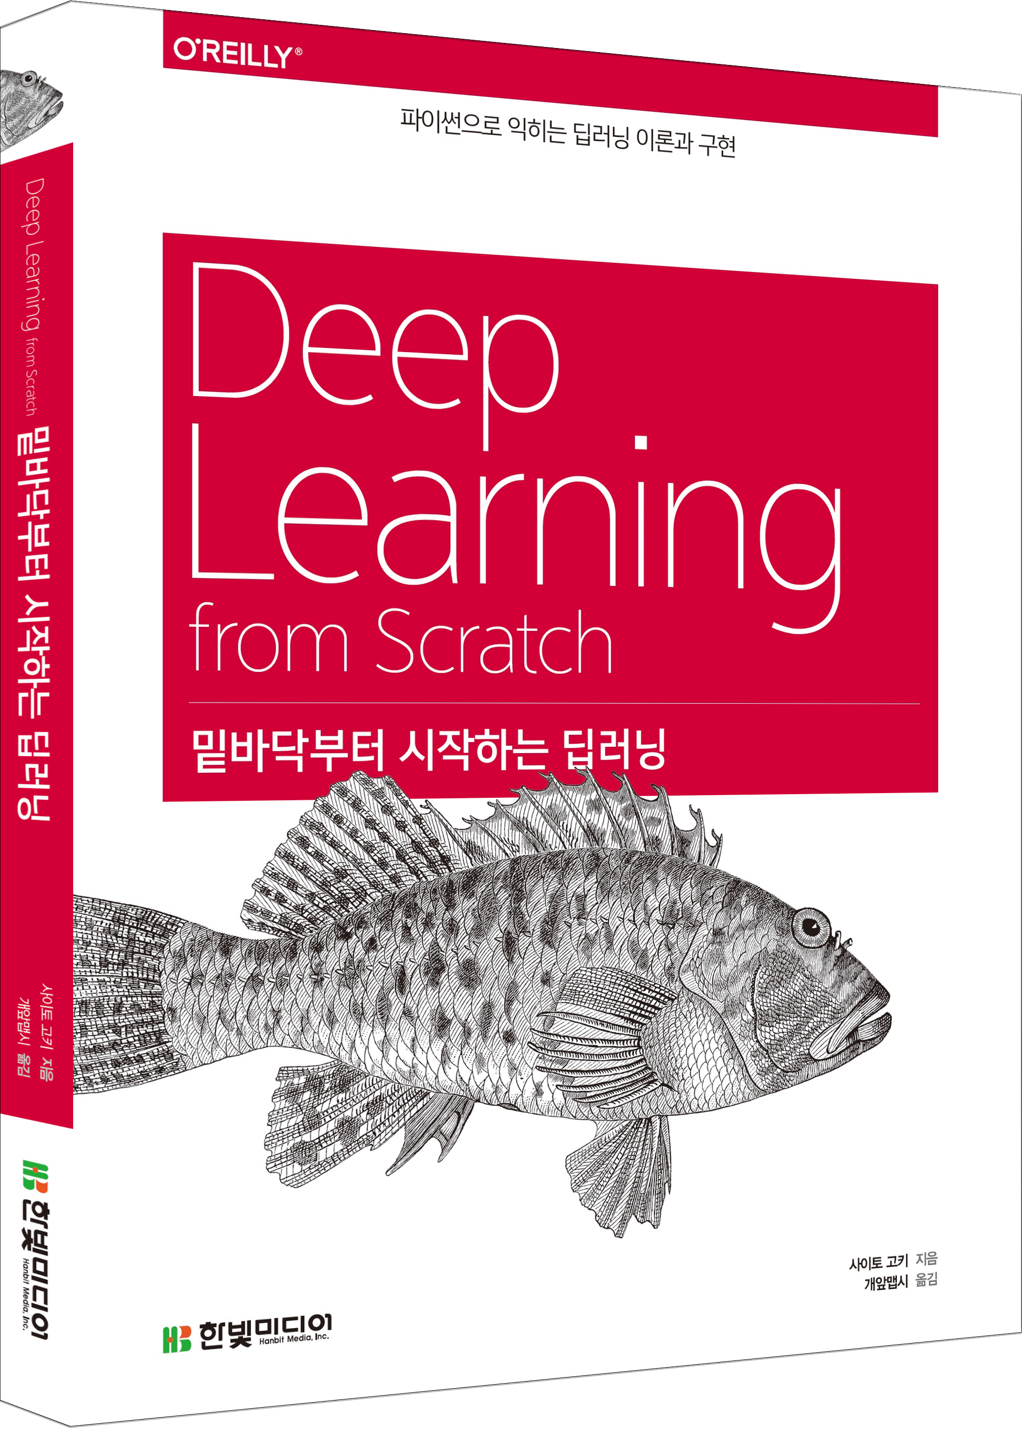
\includegraphics[width=0.5\textwidth]{fig/cover_image.jpg}
	\caption{Deep Learning의 시작으로 삼은 "Deep Learning from Scratch"}
	\label{fig:DL_book_cover}
	\end{figure}
	
	그림 \ref{fig:DL_book_cover}은 내가 deep learning을 배우기 위한 시작점으로 삼은 책이다. 이 책은 우연히 서점에서 발견한 책이고 두 가지가 문구가 나로 하여금 이 책을 선택하게 했다. 첫번째 문구는 제목에서 보인 ``from scratch'' 이다. 밑바닥 부터 시작한다는 뜻이니까, deep learning에 대해 모르는 사람들에게도 아주 기초적인 개념부터 하나씩 차근차근 설명해 주겠다는 친절한 문구이다. 그리고 실제로 내용또한 deep learning을 모르더라도 차근차근 이해할 수 있는 내용들로 구성되었다.
	
	두번째 문구는 표지 상단에 있는 ``파이썬으로 익히는''이라는 문구이다. 파이썬 덕후인 나로서 매우 반가운 문구가 아닐수 없다. 뿐만 아니라, 내용을 얼핏 보니 책의 각 장에서 설명한 개념을 친절하게도 파이썬 코드로 하나하나 설명해 줬다. 게다가 타이핑하기 귀찮으면 Github에서 clone해서 쓰란다.
	
	이러한 두 문구로 이 책을 선택했고, 읽고 내용에 감동하여 지금 이렇게 잉여력을 발휘하여 글을 쓰고 있다.
	
	\subsection{책의 간략한 구성}
	책의 1장은 파이썬의 간단한 문법과 deep learning구현을 위한 라이브러리(numpy)를 소개한다. 파이썬을 안다면 넘어가도 좋다. 혹시 안다고 해도 numpy 설명 부분은 한번쯤은 봐두자.
	
	2장은 퍼셉트론에 대해 설명한다.  퍼셉트론은 신경망에 기원이 되는 알고리즘이라서 소개 한다고 한다. 어떤가 벌써 부터 ``from scratch''라는 공약을 지키는 모습을 보여준다.
	
	3장은 이제 퍼셉트론에 활성화 함수라는 것을 덫붙이고 퍼셉트론을 여러개 붙이는 그럴싸한 신경망이란 것을 소개한다. 2장의 내용을 확장한 것이라 보면 된다. 퍼셉트론이라는 deep leaning이라는 연산의 기본 단위를 확장해서 퍼셉트론이 모이면 어떤 큰 일을 할 수 있는지를 보여준다.
	
	4장은 신경망이 어떻게 스스로 자기 자신을 개선하는지를 보여준다. 이때 손실함수, 경사 하강법이 등장한다. 손실 함수는 퍼셉트론의 각 노드에 대한 가중치로 인한 결과에 대한 정량적인 평가 방법이다. 마치 노드의 가중치를 얼마얼마 주고 답을 알고 있는 데이터로 학습 시켰을때 ``음 그렇게 가중치 주면 70점짜리 결과를 보인다.''라는 식의 결과를 산출하는 방법이다. 
	
	이렇게 손실 함수로 우리가 퍼셉트론 가중치의 학습 결과를 평가 할 수 있다면 평가 점수가 가장 높게 받을 수 있는 가중치 값을 찾으면 훌륭한 신경망을 만들 수 있게 된다. 최적의 가중치 값을 찾는 방법중 하나가 경사 하강법이다. 손실함수는 어찌 되었건 간에 퍼셉트론의 가중치 값에 대한 평가 결과를 계산하고 그것을 시각화 해보면 가중치를 각각의 차원 축으로 하는 임임의 차원 공간에 물체로 그려질 것이다. 이때 대입한 각 가중치에 대한 미분값을 통해 현재 가중치 값에서 어느 방향으로 진해하면 손실함수의 평가 결과를 좋게 받을 수 있을지를 알 수 있게 된다.
	
	정리 하자면, 4장은 신경망을 구성하는 퍼셉트론의 가중치와 그 가중치를 평가하고 개선하는 알고리즘을 소개 한다.
	
	5장은 오차역전파법이라는 괴랄한 이름의 알고리즘을 소개한다. 쉽게 말하면 4장에서 소개한 편미분을 이용한 경사 하강법이 사실은 엄청난 계산량을 요구하고 이를 개선한 방법이다. 5장은 매우 중요 하지만 전체적인 큰 흐름을 이해하고 싶다면 넘어가도 좋다.
	
	6장또한 부가적인 내용이긴 하지만 알아두면 도움이 될 것 같다. 하지만 시간이 없다면 스킵~~. 5장은 4장에서 소개한 편미분을 계산량을 획기적으로 줄이는 방법을 제시했다면 6장은 4장에서 소개한 가중치를 개선하는 전략은 경사 하강법의 보완 버전들을 소개한다. 알아두면 좋지만, 전체 흐름의 이해가 우선이라면 스킵해도 좋다.
	
	7장은 CNN이라는 합성곱 신경망을 소개한다. 요건 좀 중요한데, 앞서 신경망은 인풋 데이터를 1차원 배열로 놓고 풀지만, CNN부터는 데이터를 있는 그대로 처리하는데 초점을 맞춘다. 간단히 예를 들자면, 이미지 처리를 할경우 신경망은 2차원 이미지 데이터를 1차원 배열로 변경하여 문제를 푼다. 반면 CNN은 이미지 데이터를 있는 그대로 2차원 배열로 받아서 인식을 한다. 이를 위해 "합성곱(혹은 필터 연산이로고도 한다.)", "패딩", "스트라이드", "풀링"을 설명한다. 이 부분을 읽을때 꼭 이해해야할 중요한 컨셉이다.
	
	8장은 마지막 장으로 CNN 진화 버전으로 딥러닝이라 불리우는 다양한 기술에 대해 설명한다.
	
	정리 하자면,7장의 CNN을 설명하기 위해 2,3,4장에서 퍼셉트론, 신경망, 신경망 학습을 설명한다. CNN을 설명했으니 CNN을 이용해서 현재의 deep learning 최신 기술을 8장에서 설명할 수 있던 것이다.